\section{Looking at the backreflex}
We now placed the PD on the backreflecting light beam. So now, we expect to see dips instead of peaks in our signal.


\begin{figure}[htbp]
    \centering
    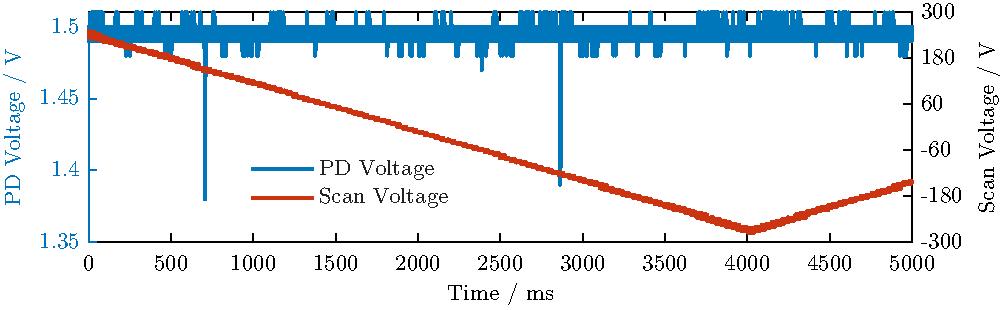
\includegraphics[width=\textwidth]{back/Figure_1.pdf}
    \caption{Here, we see dips instead of peaks. The red curve now accurately shows the piezo scan voltage. This was achievable by setting up a function generator with two synced outputs. By choosing the same settings for both outputs (12 Hz and 2.7 V peak tp peak) and then matching their phase, this signal should be an accurate representation of the piezo scan voltage.}
\end{figure}
Now, I inverted the signal in order to be able to use my existing code for further analysis. I kept the EOM running to compare the FHWM.

\begin{figure}[htbp]
    \centering
    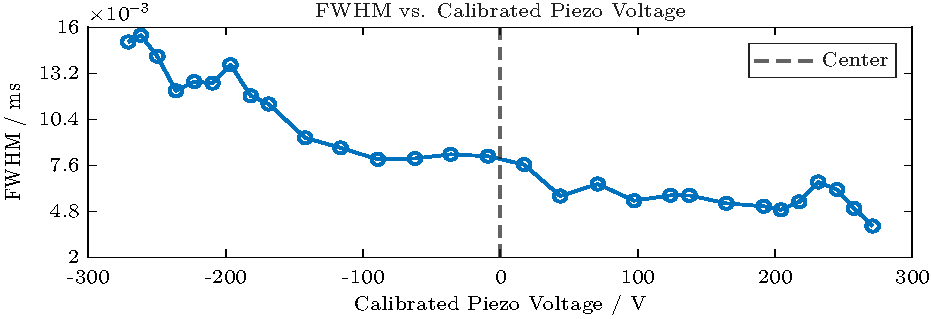
\includegraphics[width=\textwidth]{back/Figure_3.pdf}
    \caption{Zoomed in on one peak with its sidebands.}
\end{figure}
\begin{figure}[htbp]
    \centering
    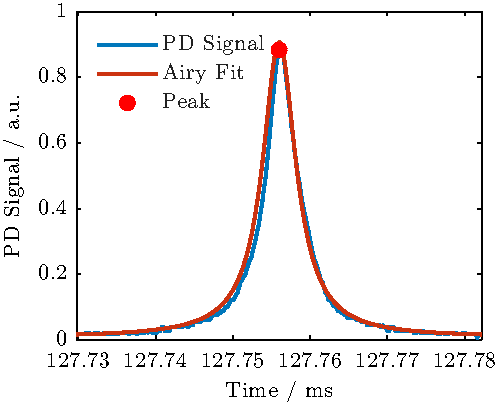
\includegraphics[width=\textwidth]{back/Figure_4.pdf}
    \caption{Zoomed in on antoher peak with its sidebands.}
\end{figure}

The FWHM values appear slightly larger than in the previous transmission setup.
However, due to the high noise level, the sideband peak detection is less accurate than before.
When the detector was placed back on the transmission side, the FWHM values matched in both cases (within 10\%). 
So perhaps the measurement in the previous section was just lucky.

The EOM was set to 10 dBm instead of the previous 12 dBm (at the transmission setup) to try to preserve the central cavity peak as much as possible. 
The EOM cuts away intensity from the central peak, which makes it harder to make out.
All in all, the backreflecting light shows similar finesse values than the transmission side. 
